% Options for packages loaded elsewhere
\PassOptionsToPackage{unicode}{hyperref}
\PassOptionsToPackage{hyphens}{url}
%
\documentclass[
  12pt,
  spanish,
]{article}
\usepackage{lmodern}
\usepackage{amssymb,amsmath}
\usepackage{ifxetex,ifluatex}
\ifnum 0\ifxetex 1\fi\ifluatex 1\fi=0 % if pdftex
  \usepackage[T1]{fontenc}
  \usepackage[utf8]{inputenc}
  \usepackage{textcomp} % provide euro and other symbols
\else % if luatex or xetex
  \usepackage{unicode-math}
  \defaultfontfeatures{Scale=MatchLowercase}
  \defaultfontfeatures[\rmfamily]{Ligatures=TeX,Scale=1}
  \setmainfont[]{Georgia}
\fi
% Use upquote if available, for straight quotes in verbatim environments
\IfFileExists{upquote.sty}{\usepackage{upquote}}{}
\IfFileExists{microtype.sty}{% use microtype if available
  \usepackage[]{microtype}
  \UseMicrotypeSet[protrusion]{basicmath} % disable protrusion for tt fonts
}{}
\makeatletter
\@ifundefined{KOMAClassName}{% if non-KOMA class
  \IfFileExists{parskip.sty}{%
    \usepackage{parskip}
  }{% else
    \setlength{\parindent}{0pt}
    \setlength{\parskip}{6pt plus 2pt minus 1pt}}
}{% if KOMA class
  \KOMAoptions{parskip=half}}
\makeatother
\usepackage{xcolor}
\IfFileExists{xurl.sty}{\usepackage{xurl}}{} % add URL line breaks if available
\IfFileExists{bookmark.sty}{\usepackage{bookmark}}{\usepackage{hyperref}}
\hypersetup{
  pdflang={es-CO},
  hidelinks,
  pdfcreator={LaTeX via pandoc}}
\urlstyle{same} % disable monospaced font for URLs
\usepackage[margin=1in]{geometry}
\usepackage{color}
\usepackage{fancyvrb}
\newcommand{\VerbBar}{|}
\newcommand{\VERB}{\Verb[commandchars=\\\{\}]}
\DefineVerbatimEnvironment{Highlighting}{Verbatim}{commandchars=\\\{\}}
% Add ',fontsize=\small' for more characters per line
\usepackage{framed}
\definecolor{shadecolor}{RGB}{248,248,248}
\newenvironment{Shaded}{\begin{snugshade}}{\end{snugshade}}
\newcommand{\AlertTok}[1]{\textcolor[rgb]{0.94,0.16,0.16}{#1}}
\newcommand{\AnnotationTok}[1]{\textcolor[rgb]{0.56,0.35,0.01}{\textbf{\textit{#1}}}}
\newcommand{\AttributeTok}[1]{\textcolor[rgb]{0.77,0.63,0.00}{#1}}
\newcommand{\BaseNTok}[1]{\textcolor[rgb]{0.00,0.00,0.81}{#1}}
\newcommand{\BuiltInTok}[1]{#1}
\newcommand{\CharTok}[1]{\textcolor[rgb]{0.31,0.60,0.02}{#1}}
\newcommand{\CommentTok}[1]{\textcolor[rgb]{0.56,0.35,0.01}{\textit{#1}}}
\newcommand{\CommentVarTok}[1]{\textcolor[rgb]{0.56,0.35,0.01}{\textbf{\textit{#1}}}}
\newcommand{\ConstantTok}[1]{\textcolor[rgb]{0.00,0.00,0.00}{#1}}
\newcommand{\ControlFlowTok}[1]{\textcolor[rgb]{0.13,0.29,0.53}{\textbf{#1}}}
\newcommand{\DataTypeTok}[1]{\textcolor[rgb]{0.13,0.29,0.53}{#1}}
\newcommand{\DecValTok}[1]{\textcolor[rgb]{0.00,0.00,0.81}{#1}}
\newcommand{\DocumentationTok}[1]{\textcolor[rgb]{0.56,0.35,0.01}{\textbf{\textit{#1}}}}
\newcommand{\ErrorTok}[1]{\textcolor[rgb]{0.64,0.00,0.00}{\textbf{#1}}}
\newcommand{\ExtensionTok}[1]{#1}
\newcommand{\FloatTok}[1]{\textcolor[rgb]{0.00,0.00,0.81}{#1}}
\newcommand{\FunctionTok}[1]{\textcolor[rgb]{0.00,0.00,0.00}{#1}}
\newcommand{\ImportTok}[1]{#1}
\newcommand{\InformationTok}[1]{\textcolor[rgb]{0.56,0.35,0.01}{\textbf{\textit{#1}}}}
\newcommand{\KeywordTok}[1]{\textcolor[rgb]{0.13,0.29,0.53}{\textbf{#1}}}
\newcommand{\NormalTok}[1]{#1}
\newcommand{\OperatorTok}[1]{\textcolor[rgb]{0.81,0.36,0.00}{\textbf{#1}}}
\newcommand{\OtherTok}[1]{\textcolor[rgb]{0.56,0.35,0.01}{#1}}
\newcommand{\PreprocessorTok}[1]{\textcolor[rgb]{0.56,0.35,0.01}{\textit{#1}}}
\newcommand{\RegionMarkerTok}[1]{#1}
\newcommand{\SpecialCharTok}[1]{\textcolor[rgb]{0.00,0.00,0.00}{#1}}
\newcommand{\SpecialStringTok}[1]{\textcolor[rgb]{0.31,0.60,0.02}{#1}}
\newcommand{\StringTok}[1]{\textcolor[rgb]{0.31,0.60,0.02}{#1}}
\newcommand{\VariableTok}[1]{\textcolor[rgb]{0.00,0.00,0.00}{#1}}
\newcommand{\VerbatimStringTok}[1]{\textcolor[rgb]{0.31,0.60,0.02}{#1}}
\newcommand{\WarningTok}[1]{\textcolor[rgb]{0.56,0.35,0.01}{\textbf{\textit{#1}}}}
\usepackage{graphicx,grffile}
\makeatletter
\def\maxwidth{\ifdim\Gin@nat@width>\linewidth\linewidth\else\Gin@nat@width\fi}
\def\maxheight{\ifdim\Gin@nat@height>\textheight\textheight\else\Gin@nat@height\fi}
\makeatother
% Scale images if necessary, so that they will not overflow the page
% margins by default, and it is still possible to overwrite the defaults
% using explicit options in \includegraphics[width, height, ...]{}
\setkeys{Gin}{width=\maxwidth,height=\maxheight,keepaspectratio}
% Set default figure placement to htbp
\makeatletter
\def\fps@figure{htbp}
\makeatother
\setlength{\emergencystretch}{3em} % prevent overfull lines
\providecommand{\tightlist}{%
  \setlength{\itemsep}{0pt}\setlength{\parskip}{0pt}}
\setcounter{secnumdepth}{5}
\usepackage{dcolumn}
\usepackage{rotating}
\usepackage{xcolor}
\usepackage[bottom]{footmisc}
\usepackage{setspace}
\usepackage{multirow}
\usepackage{footnote}
\usepackage{booktabs}
\usepackage{longtable}
\usepackage{array}
\usepackage{multirow}
\usepackage{wrapfig}
\usepackage{float}
\usepackage{colortbl}
\usepackage{pdflscape}
\usepackage{tabu}
\usepackage{threeparttable}
\usepackage{threeparttablex}
\usepackage[normalem]{ulem}
\usepackage{makecell}
\usepackage{xcolor}
\ifxetex
  % Load polyglossia as late as possible: uses bidi with RTL langages (e.g. Hebrew, Arabic)
  \usepackage{polyglossia}
  \setmainlanguage[]{spanish}
\else
  \usepackage[shorthands=off,main=spanish]{babel}
\fi

\author{}
\date{\vspace{-2.5em}}

\begin{document}

\newpage
\begin{spacing}{0.9} 
\tableofcontents
\end{spacing}

\newpage

\begin{spacing}{0.9} 
\listoftables
\end{spacing}

\newpage
\listoffigures
\newpage
\normalsize

\hypertarget{presentaciuxf3n}{%
\section{Presentación}\label{presentaciuxf3n}}

Tradicionalmente, los procesamientos estadísticos en el INE han
recurrido a una estrategia de codificación manual para analizar las
respuestas a variables de preguntas abiertas. De este modo, personas
entrenadas en el uso de clasificadores leen cada uno de los registros y
asignan el código más adecuado, sobre la base de criterios predefinidos.
Este procedimiento, por ser intensivo en trabajo manual, requiere una
gran cantidad de tiempo y presenta algunas limitaciones para lograr una
completa uniformidad en la utilización de criterios.

Con el objeto de hacer más eficiente el uso de recursos y mejorar la
calidad de los datos, durante los últimos años la institución ha
avanzado en estrategias automatizadas de codificación, basadas en
técnicas de aprendizaje de máquinas (\emph{machine learning}). El
conocimiento acumulado y el desarrollo de competencias han permitido que
estas técnicas sean aplicadas en la Encuesta Nacional de Empleo (ENE),
en la Encuesta Nacional de Seguridad Ciudadana 2019 (ENUSC) y en la
última Prueba Piloto de la Encuesta de Presupeustos Familiares
(realizada en 2020). En el caso de la ENE, desde marzo de 2019 se está
implementando una metodología similar a la desarrollada por Guerrero y
Cabezas (Cabezas, J. y Guerrero, J. 2019), quienes muestran resultados
para CAENES y CIUO-88.CL\footnote{CAENES corresponde al acrónimo de
  Clasificador de Actividades Económicas Nacional para Encuestas
  Sociodemográficas. Este clasificador es una adaptación de la
  Clasificación industrial internacional uniforme (CIIU), creado para
  facilitar la medición de actividad económica en el contexto de
  encuestas de hogares. CAENES es utilizado en el INE desde 2016 y su
  metodología se describe extensamente en el documento Clasificador de
  Actividades Económicas Nacional para Encuestas Sociodemográficas (INE
  2016). Por su parte, CIUO-88 corresponde al acrónimo de Clasificador
  Internacional Uniforme de Ocupaciones. En el caso del documento citado
  de Guerrero y Cabezas (2019), se utilizan datos codificados con la
  versión 88 del clasificador. Actualmente, el INE realiza sus
  levantamientos con la versión 08.}. La posterior adaptación e
implementación de dicha metodología se encuentra descrita en el
documento ``Sistema de clasificación y codificación automática en la
Encuesta Nacional de Empleo'' (INE 2019). En el caso de la Prueba Piloto
EPF, se utilizaron modelos de \emph{deep learning} para codificar los
datos de gasto en base al clasificador CCIF. Por su parte, en ENUSC 2019
se automatizó la codificación de CIUO-08.CL, también mediante una
estrategia basada en \emph{machine learning}.

Sin duda, la utilización de este tipo de herramientas supone un avance
en la elaboración de estadísticas, ya que ello permite disminuir tiempos
de procesamiento y mejorar la calidad de los productos, sin embargo, los
métodos de clasificación basados en \emph{machine learning} presentan
algunas limitaciones que no deben perderse de vista. Una de las más
importantes guarda relación con la posible desactualización de los datos
que se utilizan para el entrenamiento de los modelos.

Cuando los datos de entrenamiento comienzan a perder representatividad
o, dicho de otro modo, cuando las características del conjunto de
entrenamiento empiezan a diferir de manera importante de las
características de los datos para los cuales se busca hacer una
predicción, lo más probable es que el rendimiento real sea más bajo que
el estimado durante el proceso de entrenamiento. En la medida en que los
nuevos datos se van distanciando del conjunto inicial, lo esperable es
que las predicciones se vayan deteriorando progresivamente, afectando de
manera importante la calidad estadística de los productos que usen esta
estrategia.

La desactualización puede provenir de varias fuentes. Una de las más
importantes se relaciona con cambios metodológicos, tales como el
tránsito de encuestas en papel a dispositivos electrónicos,
modificaciones en los cuestionarios, incorporación de nuevas
instrucciones en los operativos de campo, entre otras. Una segunda
fuente de desactualización es el dinamismo propio de los fenómenos que
las encuestas de hogares miden. A modo de ejemplo, tanto la ocupación
como el consumo de los hogares constituyen fenómenos que van cambiando
en el tiempo. Así, al alero de cambios tecnológicos, van surgiendo
nuevas ocupaciones, a la vez que otras desaparecen. En el caso del
consumo de los hogares ocurre algo similar, ya que el mercado
constantemente va cambiando la oferta de bienes y servicios, al mismo
tiempo que se modifican las preferencias de los hogares.

Todos estos cambios añaden dificultades a las estrategias de
codificación basadas en técnicas de \emph{machine learning} e imponen la
necesidad de monitorear constantemente los modelos que están en
producción, con el objeto de introducir ajustes, en caso de que ello sea
necesario. En ese sentido, el presente proyecto tiene como objetivo
principal construir bases de entrenamiento actualizadas y optimizar
algoritmos de codificación automatizada para los clasificadores CAENES y
CIUO-08.CL. Dado que la institución se encuentra en un proceso de
migración hacia dispositivos electrónicos de captura, es deseable contar
con datos de entrenamiento que provengan de levantamientos con
dispositivos de este tipo. El motivo de ello es que la manera en la que
se registra la información en un dispositivo electrónico difiere del
modo en que las personas lo hacen en un formato basado en papel, en
términos de cantidad y tipo de palabras utilizadas. Es así que el
presente proyecto pone a disposición dos sets de datos (CAENES y
CIUO-08.CL) provenientes de levantamientos CAPI (\emph{Computer assisted
personal interview}). En la elaboración de estos sets de entrenamiento,
se han introducido altos estándares de exigencia, con el objeto de
ofrecer datos de calidad, que permitan llevar a cabo próximos
entrenamientos.

Como objetivo secundario, este documento busca aportar a la incipiente
diseminación respecto al desarrollo y uso de técnicas basadas en
\emph{machine learning} dentro de la institución. Si bien se han llevado
a cabo avances importantes en esta materia, aún existe una brecha de
competencias que es posible estrechar. Para ello, se disponibilizan las
rutinas utilizadas en un repositorio público y al mismo tiempo se pone
en funcionamiento una herramienta (API) que permite utilizar los modelos
entrenados de manera relativamente sencilla. Con esto último se busca
que los esfuerzos realizados por este equipo puedan ser de utilidad para
operaciones que tengan necesidades similares de codificación,
contribuyendo a un uso más eficiente de los recursos públicos.

El presente documento tiene como objetivo documentar el proceso de
creación de bases de datos de entrenamiento para CAENES y CIUO-08.CL,
así como describir los principales procedimientos realizados durante la
fase de entrenamiento de los modelos. Con esto se busca poner a
disposición un material de apoyo, para quienes utilicen los datos y/o
modelos generados en el marco de este proyecto.

\newpage

\hypertarget{agradecimientos}{%
\section{Agradecimientos}\label{agradecimientos}}

Este proyecto, en particular en su fase de creación de datasets de
entrenamiento para los clasificadores CAENES y CIUO-08.CL, se benefició
de la valiosa colaboración de diferentes equipos del Instituto Nacional
de Estadísticas. El Proyecto Estratégico Servicios Compartidos para la
Producción Estadística agradece al Subdepartamento de Estadísticas
Continuas del Trabajo y al Subdepartamento de Estadísticas
Socioeconómicas por la provisión de glosas desde sus operaciones
estadísticas para construcción de los datasets de entrenamiento, y al
Departamento de Estadísticas Demográficas y Sociales, al Departamento de
Estadísticas Económicas, al Departamento de Estadísticas de Trabajo y al
Departamento de Operaciones de Estadísticas Económicas y Precios, por el
apoyo de sus profesionales en el etiquetado manual de glosas de
ocupación y actividad económica.

Se destaca especialmente el trabajo de Antonieta Maulén, analista del
Departamento de Operaciones de Estadísticas Sociales, por su dedicación
y soporte constante al proyecto, así como también a la Sección de
Nomenclaturas, del Subdepartamento de Calidad y Estándares, quienes
velaron por la calidad de la codificación de los datasets de
entrenamiento, a partir de auditorías y retroalimentación constante.

\newpage

\hypertarget{machine-learning-para-la-codificaciuxf3n-de-caenes-y-ciuo-08.cl}{%
\section{\texorpdfstring{\emph{Machine learning} para la codificación de
CAENES y
CIUO-08.CL}{Machine learning para la codificación de CAENES y CIUO-08.CL}}\label{machine-learning-para-la-codificaciuxf3n-de-caenes-y-ciuo-08.cl}}

\hypertarget{codificaciuxf3n-automatizada-de-textos}{%
\subsection{Codificación automatizada de
textos}\label{codificaciuxf3n-automatizada-de-textos}}

Las encuestas de hogares suelen contener preguntas abiertas en formato
de texto libre. Esta información puede tener relación con el mercado del
trabajo, el consumo de los hogares, la victimización, entre otros. Para
que dicha información sea utilizada con fines estadísticos se debe
recurrir a algún sistema de codificación estandarizado, de manera tal de
que cada texto sea asociado a un código dentro de un sistema de
clasificación. Históricamente, este trabajo ha sido realizado por
codificadores entrenados para esta tarea. Así, personas que conocen en
detalle los clasificadores leen cada uno de los textos y asignan un
código conforme a criterios pre establecidos. Esta estrategia, por
tanto, es intensiva en trabajo manual.

Es posible identificar, al menos, 2 debilidades de una estrategia basada
en codificación manual:

\begin{itemize}
\item
  Requiere una gran cantidad de tiempo, ya que es necesario que cada uno
  de los textos sea leído y luego codificado por una persona.
  Típicamente, una muestra tiene varios miles de registros, lo que
  implica que el trabajo manual destinado a esta tarea sea
  significativo, generando tiempos de espera y costos en horas persona.
\item
  El hecho de que la asignación de códigos descanse en las decisiones de
  distintas personas, hace complejo el aseguramiento de la aplicación de
  criterios uniformes. Si bien cada clasificador cuenta con un marco
  conceptual definido, la aplicación de criterios en la práctica no
  siempre resulta una tarea sencilla. La información recolectada en
  terreno muchas veces puede ser insuficiente o ambigua, lo cual hace
  que se torne difícil la utilización de criterios rígidos.
\end{itemize}

A raíz de las dos situaciones mencionadas, es deseable la utilización de
estrategias automáticas de codificación, pues estas permiten disminuir
significativamente las horas empleadas para dicha tarea y reducir el
espacio para la discrecionalidad al momento de asignar un código.

En lo que respecta a la automatización de la codificación en producción
de estadísticas oficiales, es posible identificar dos enfoques
principales: codificación basada en reglas y codificación basada en
métodos de aprendizaje de máquinas (\emph{machine learning}). En el
primero de estos enfoques, se generan reglas \emph{a priori}, mediante
las cuales un programa o rutina asigna un código. La mayor fortaleza de
este enfoque radica en que no es necesario contar con datos históricos,
pues solo se requiere que el o la analista identifique las reglas y las
programe en una rutina. Una vez realizada la tarea de identificación de
reglas, los datos pasan a través del programa y el código es asignado.
La desventaja más importante y evidente es que se hace necesario que
alguien escriba las reglas, lo cual puede constituir una tarea ardua, ya
que por lo general el número de condiciones que se deben escribir no es
despreciable. De hecho, es muy poco probable que se llegue a codificar
el 100\% de los registros mediante esta estrategia.

El segundo enfoque está basado en el aprendizaje que un algoritmo puede
obtener de los datos que se han etiquetado manualmente en el pasado. A
diferencia de la estrategia anterior el o la analista no crea las
reglas, sino que estas son aprendidas por un algoritmo, el cual, después
de un proceso de entrenamiento, es capaz de codificar registros nuevos
gracias al aprendizaje previo. Naturalmente, esta estrategia supone la
existencia de datos codificados con anterioridad, lo cual no siempre
ocurre o no ocurre de manera óptima. Por ejemplo, es posible que la
cantidad de datos codificados sea pequeña, que estos no sean
representativos del fenómeno en cuestión o que, simplemente, la calidad
del etiquetado no sea la adecuada. En cada uno de estos casos se ve
afectada la posibilidad de que un algoritmo ``aprenda'' correctamente.
Ahora bien, cuando la fuente de datos de entrenamiento sí cumple ciertos
requisitos de calidad, se puede llevar a cabo un proceso de aprendizaje,
mediante el cual es posible codificar registros nuevos en poco tiempo y
a un costo muy bajo.

Dependiendo del contexto y de los datos históricos con los que se
cuente, un equipo debería privilegiar una estrategia u otra. \emph{A
priori}, no es tan sencillo determinar qué estrategia es la más
eficiente, ya que existen consideraciones de costos que deben ser
sopesadas en el marco de cada proceso de producción estadística. Para
operaciones estadísticas coyunturales, cuya metodología no experimenta
cambios importantes, puede ser de gran utilidad un enfoque basado en
\emph{machine learning}, ya que un mismo entrenamiento puede ser
utilizado para muchas recolecciones. Por otro lado, operaciones
estadísticas de naturaleza estructural, posiblemente, no se vean
demasiado benefiadas por una estrategia de \emph{machine learning}, ya
que en periodos extensos de tiempo es muy problable que los
clasificadores experimenten cambios relevantes, lo cual dejaría en
obsolecencia los datos de entrenamiento.

El INE cuenta con experiencia institucional en el uso de ambos enfoques,
sin embargo, en lo que respecta al presente documento, se ahondará
solamente en la estrategia de \emph{machine learning}.

\hypertarget{limitaciones-de-un-muxe9todo-de-machine-learning}{%
\subsection{\texorpdfstring{Limitaciones de un método de \emph{machine
learning}}{Limitaciones de un método de machine learning}}\label{limitaciones-de-un-muxe9todo-de-machine-learning}}

Una codificación automática basada en \emph{machine learning} tiene una
serie de ventajas, sin embargo, también presenta algunas limitaciones
que es preciso tener en consideración al momento de poner en producción
esta estrategia. El supuesto más importante en una estrategia basada en
\emph{machine learning} es que los datos de entrenamiento son
representativos de los datos nuevos que se pretende codificar. Si dicho
supuesto no se cumple, la estimación del error de predicción estará
sesgada y, muy probablemente, el error real sea mayor al estimado. En
ese sentido, nunca debe perderse de vista la relación que existe entre
los datos de entrenamiento y aquellos para los que se está haciendo una
predicción. En el contexto de las estadísticas oficiales, este problema
podría originarse por varias causas. Algunas de las más importantes son:

\begin{itemize}
\item
  El dinamismo de los fenómenos en cuestión: la ocupación, el consumo o
  la producción son fenómenos que van cambiando constantemente. En el
  caso del mercado del trabajo, es posible que surjan nuevas ocupaciones
  que no estén consideradas dentro del conjunto de datos de
  entrenamiento. Un ejemplo de ello son las ocupaciones que surgen al
  alero de cambios técnológicos. En el caso del consumo de los hogares
  ocurre algo similar, ya que constantemente nuevos bienes y servicios
  son lanzados al mercado, lo que introduce presión sobre el proceso de
  codificación automática.
\item
  Cambios metodológicos durante la recolección: podría ocurrir que los
  elementos que componen el modo de captura sean modificados y ello
  introduzca cambios en las características de los datos. Algunos
  ejemplos de ello son: cambios en las baterías de preguntas utilizadas
  o en su fraseo, migración de papel a dispositivos móviles de captura,
  cambio en las instrucciones por parte de los equipos de terreno, entre
  otros. Todas estas situaciones podrían generar un cambio en el modo en
  el que se registra la información, haciendo que los nuevos datos se
  distancien de aquellos utilizados en el entrenamiento.
\end{itemize}

Si comienza a generarse una distancia considerable entre los datos de
entrenamiento y aquellos para los que se pretende hacer una predicción,
es posible que el rendimiento estimado inicialmente vaya disminuyendo
progresivamente. Es deseable, entonces, contar con herramientas que
permitan identificar cuándo la predicción del modelo comienza a
disminuir. Ahora bien, la identificación de dicho punto no es trivial.
La manera más sencilla, pero al mismo tiempo más costosa, es la revisión
periódica de las predicciones del modelo por parte de personal altamente
entrenado en el sistema de clasificación. Con ello se busca comparar la
predicción del modelo con algo que en el contexto de \emph{machine
learning} se suele llamar \emph{ground truth}, es decir, con una
codificación considerada correcta. En este caso, se asume que los
códigos asignados por una persona experta son la \emph{ground truth}. Si
una estrategia como esta se realiza con la periodicidad adecuada, es
posible identificar el momento en el cual la precisión del modelo
comienza a disminuir. La limitación más importante es que se requiere
contar con recursos humanos altamente especializados para esta tarea,
sin embargo, es importante mencionar que dichos costos siempre son
menores a los de codificar todos los registros manualmente.

Una segunda alternativa sería implementar un sistema automatizado que
genere una métrica que compare las características de los datos de
entrenamiento con aquellos para los que se requiere una predicción. Esta
métrica opera como un \emph{proxy} de precisión, lo cual permite
moniteorear el rendimiento del modelo por medio de una variable que no
es la precisión, pero que sí se relaciona con ella.

Independientemente de la estrategia para hacer el seguimiento del
modelo, la acción esperada es una revisión del proceso de entrenamiento.
En ciertas ocasiones el problema podría solucionarse con ciertos ajustes
en el procedimiento, pero si el problema se explica por un cambio
importante en los datos nuevos respecto a los de entrenamiento, es
decir, por una pérdida de representatividad de estos últimos, la
alternativa más adecuada es la adición de un conjunto nuevo de datos
etiquetados manualmente, es decir, la amplicación de la base de
entrenamiento.

\hypertarget{generaciuxf3n-de-los-conjuntos-de-datos-de-entrenamiento}{%
\section{Generación de los conjuntos de datos de
entrenamiento}\label{generaciuxf3n-de-los-conjuntos-de-datos-de-entrenamiento}}

\hypertarget{principales-fuentes-de-informaciuxf3n-y-codificaciuxf3n}{%
\subsection{Principales fuentes de información y
codificación}\label{principales-fuentes-de-informaciuxf3n-y-codificaciuxf3n}}

Dado que uno de los objetivos del proyecto era generar conjuntos de
datos etiquetados provenientes de encuestas realizadas mediante CAPI,
las principales fuentes de información corresponden a dicha modalidad.
Dos son las fuentes de información más importantes: 1) coyuntura ENE
entre los meses de junio y noviembre de 2020, provenientes del sistema
informático de la encuesta, que es el que aloja los datos de
recolecciones realizadas mediante dispositivo móvil de captura y 2)
encuesta Piloto EPF 2020. Una tercera fuente de información muy marginal
corresponde a la coyuntura ENE del año 2018, pero solo para algunas
categorías de CAENES, escasamente representadas en la base de datos
construida inicialmente.

Respecto al origen de la codificación, la mayor parte de esta fue
realizada por un equipo de codificadores y codificadoras que apoyaron
las actividades del Proyecto Estratégico Servicios Compartidos para la
Producción Estadística. Dicho equipo etiquetó datos provenientes de la
coyuntura ENE entre los meses de junio y noviembre de 2020. Una segunda
fuente de etiquetado corresponde al control de calidad realizado por el
Departamento de Estudios del Trabajo (DET) en el marco de la coyuntura
de la Encuesta de Empleo. Debido a que estos datos ya habían sido
revisados por una analista experta, pasaron directamente a formar parte
del dataset de entrenamiento.

\hypertarget{proceso-de-etiquetado-manual}{%
\subsection{Proceso de etiquetado
manual}\label{proceso-de-etiquetado-manual}}

\hypertarget{codificaciuxf3n-cruzada}{%
\subsubsection{Codificación cruzada}\label{codificaciuxf3n-cruzada}}

Con el objeto de alcanzar una codificación de alta calidad se implementó
un sistema de doble etiquetado. Así, al principio del proceso cerca de
un 90\% de los datos fue codificado por dos analistas diferentes, con el
fin de conseguir una mayor seguridad respecto al código asignado para
cada glosa. Cuando se producía una diferencia en el código asignado, un
tercer analista más calificado, discernía cuál era el código final. Es
importante mencionar que el porcentaje de doble codificación fue
disminuyendo cuando se detectó que la cantidad de registros con
discrepancias comenzó a decaer. La decisión de diminuir el porcentaje de
doble codificación obedece a motivos de costos, ya que para cumplir con
los objetivos del proyecto, se hizo necesario aumentar la velocidad de
codificación.

Es relevante señalar que durante todo el proceso de codificación se
contó con el apoyo de la Sección de Nomenclaturas, dependiente del
Subdepartamento de Calidad y Estándares, quienes revisaban una muestra
mensual de aproximadamente 150 registros para cada clasificador. A
partir de dicha revisión, se retroalimentaba al equipo de codificación,
tanto en CAENES como en CIUO-08.CL. Esto permitió rectificar ciertos
criterios y revisar algunos registros que habían sido codificados sobre
la base de reglas mal implementadas. Cabe señalar que las auditorías no
solo cumplieron la función de retroalimentación sino que, además, se
utilizaron para mejorar la calidad de la codificación, ya que para todos
los casos que fueron seleccionados para auditar, el código asignado por
el equipo del proyecto estratégico fue reemplazado por el asignado por
la Sección de Nomenclaturas.

Los siguientes gráficos muestran el porcentaje de coincidencia entre el
equipo de codificación del proyecto y la Sección de Nomenclaturas a lo
largo del periodo de trabajo. En el caso de CIUO-08.CL, se advierte un
aumento importante de la coincidencia en un breve periodo de tiempo. Por
otro lado, en CAENES la precisión se mantiene relativamente estable y la
caída que se observa durante el tercer mes es atribuible a un efecto de
la muestra escogida, pues al ser esta de solo 150 casos, es esperable
encontrar variaciones de este nivel entre muestras, lo cual lleva a
desestimar una caída real en el rendimiento en el mes en cuestión. De
hecho, en la auditoría final, como se mostrará en el siguiente apartado,
se registra una precisión de 92,5\% aproximadamente en la codificación
de CAENES.

Una de las razones más importantes que explican las trayectorias
disímiles de ambos clasificadores se relaciona con la experiencia de las
personas que trabajaron en cada uno de los clasificadores. En el caso de
CAENES participaron analistas que contaban con experiencia realizando
esta tarea, de modo que el espacio de mejora era más limitado que en el
caso de CIUO-08.CL, cuyos codificadores y codificadoras no contaban con
experiencia previa ni conocían el clasificador, lo que implicaba un
espacio de mejora más amplio\footnote{Todas las personas que colaboraron
  en la codificación de los datasets de entrenamiento participaron de
  una capacitación inicial implementada por la Sección de Nomenclaturas.
  La experiencia previa en codificación, si bien era deseable, no fue un
  atributo exigible, dada la dificultad de conseguir apoyos con dicha
  especialización.} .

\begin{figure}[H]
\centering
\large
\caption{Porcentaje de coincidencia entre equipo de codificación y Sección de Nomenclaturas para CIUO-08.CL y CAENES}
\label{div_ic_nac}
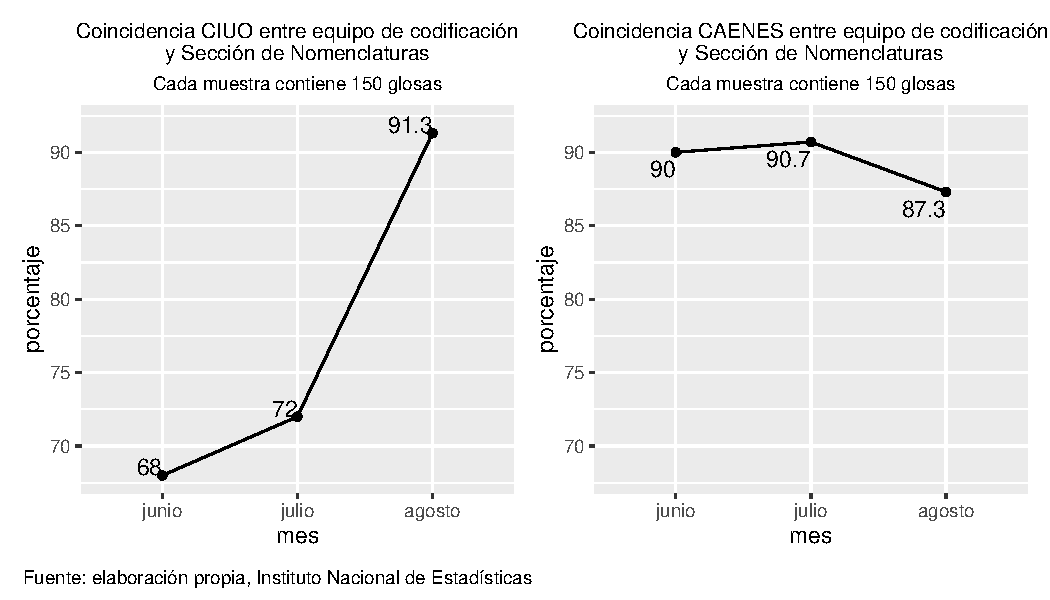
\includegraphics[width = \linewidth]{imagenes/auditorias_parciales.pdf}
\normalsize
\end{figure}

Las siguientes figuras muestran fragmentos del tablero utilizado para
retroalimentar al equipo de codificación, sobre la base de la
información proporcionada por la auditoría de la Sección de
Nomenclaturas. Mediante esta herramienta se informaba cuáles eran los
códigos que tenían mayor número de errores y en qué consistían dichos
errores. El tablero contenía información personalizada para cada miembro
del equipo, lo que permitía hacer una retroalimentacion a un nivel
individualizado, a fin de implementar los ajustes necesarios. Los dos
gráficos de más abajo fueron la herramienta más utilizada durante este
proceso, pues permitían conocer cuáles eran los códigos que generaban
mayor confusión. A modo de ejemplo, el gráfico de abajo a la derecha da
cuenta de que el código 92 se estaba confundiendo con los códigos 43,
75, 81 y 93. Esta información fue de gran ayuda para identificar
desviaciones en los criterios del clasificador, ya que muchas veces
existen sutilezas difíciles de incorporar, que determinan la pertenencia
de una glosa a uno u otro subgrupo principal.

\begin{figure}[H]
\centering
\large
\caption{Dashboard para el seguimiento del avance de codificación}
\label{ciuo_distancia}
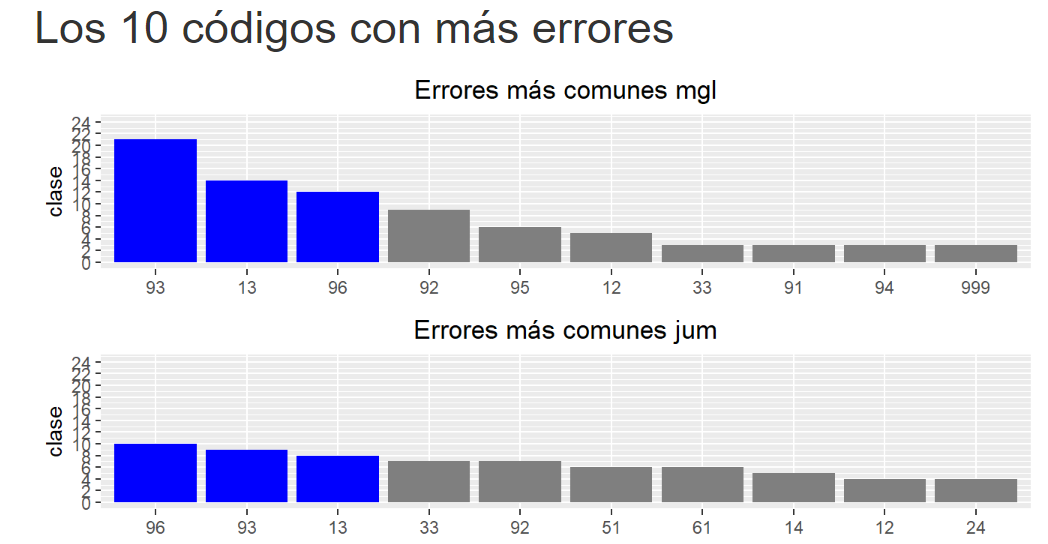
\includegraphics[width = \linewidth]{imagenes/resumen_errores.png}
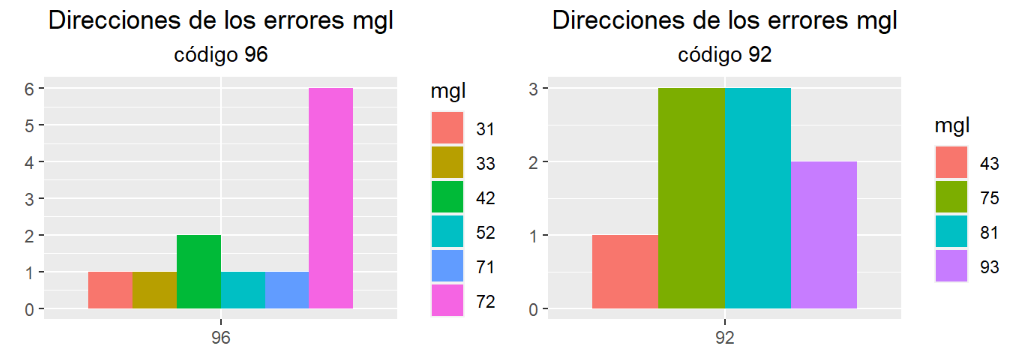
\includegraphics[width = \linewidth]{imagenes/direccion_errores.png}
\normalsize
\end{figure}

Debido a que el equipo de codificación estaba conformado por personas
con disponibilidades de tiempo variadas, era importante contar con algún
sistema de seguimiento que permitiera conocer el nivel de avance del
proyecto semana a semana. Para ello, se implementó un tablero que
permitía monitorear la cantidad de registros codificados por cada
persona, así como su nivel de cumplimiento, según la productividad
esperada. Las visualizaciones permitían identificar en tiempo real el
momento en el que comenzaban a producirse atrasos, lo cual hacía posible
llevar a cabo reasignaciones de carga en los casos en los que era
necesario. A modo de ejemplo, el gráfico superior derecho muestra que la
primera semana se esperaban 600 registros codificados, sin embargo,la
cantidad de glosas en ese momento era 0, lo cual evidenciaba un retraso
en el trabajo planificado. Este tablero se actualizaba de manera
automática una vez por día y estaba disponible para cada uno de los y
las integrantes del equipo. Las líneas horizontales representaban
semanas de trabajo y cambiaban de color, a fin de mostrar la cantidad de
tiempo transcurrido desde la entrega de la asignación.

\begin{figure}[H]
\centering
\large
\caption{Dashboard para el seguimiento del avance de codificación}
\label{avance_codificacion}
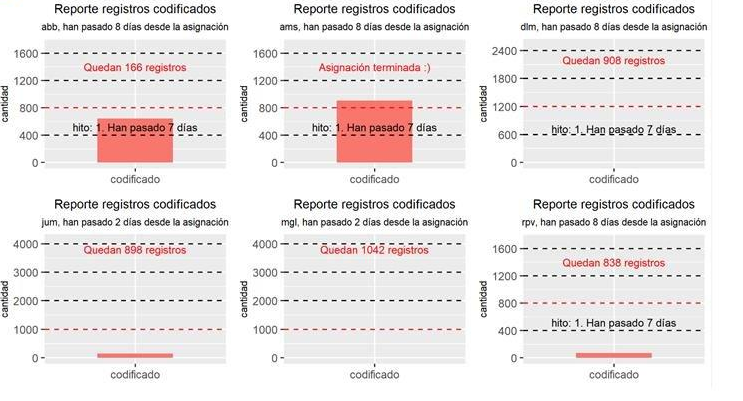
\includegraphics[width = \linewidth]{imagenes/avance_codificacion.png}
\normalsize
\end{figure}

\hypertarget{revisiuxf3n-de-cuxf3digos-complejos}{%
\subsubsection{Revisión de códigos
complejos}\label{revisiuxf3n-de-cuxf3digos-complejos}}

Sobre la base de la información recolectada de la codificación cruzada y
de las auditorías, se tomó la decisión de llevar a cabo una revisión
masiva de algunos códigos complejos. Para el caso de CIUO-08.CL, la
Sección de Nomenclaturas revisó 2.000 registros.

En el caso de CAENES se realizaron dos revisiones. En primer lugar,
15.318\footnote{Existen tres motivos que explican la diferencia en el
  número de casos revisados en cada uno de los clasificadores En primer
  lugar, el dataset de CAENES está compuesto por prácticamente el doble
  de registros que el de CIUO-08.CL. En segundo lugar, la complejidad de
  CIUO-08 impone la restricción de minimizar el número de glosas
  revisadas, ya que el tiempo requerido es considerablemente mayor.
  Finalmente, en el caso de CAENES, el equipo contaba con una analista
  muy experimentada que colaboró durante algunas semanas con una
  fracción importante de su jornada laboral. Ello no ocurrió en el caso
  de CIUO-08, cuya revisión estuvo a cargo de la Sección de
  Nomenclaturas y, por ende, sujeta a las restricciones de tiempo de
  dicho equipo.} registros pertenecientes a códigos complejos. En
segundo lugar, se revisaron 5.904 registros que cumplían con la
característica de tener glosas idénticas, pero con códigos diferentes.
Lo anterior requiere un comentario, pues el hecho de que dos glosas
idénticas tengan códigos diferentes no necesariamente constituye un
error. De acuerdo a la metodología institucional, la primera fuente de
información para codificar debe ser la glosa, sin embargo, existen casos
en los que la información contenida en ella no permite asignar un código
con precisión, a raíz de lo cual se recurre a variables auxiliares. Esto
quiere decir que dos glosas idénticas podrían llegar a tener códigos
diferentes, si la información de las variables auxiliares así lo
sugiere. De hecho, una parte importante de los registros revisados por
esta situación no tuvo modificación\footnote{Las preguntas principales
  para codificar CAENES son c5, c9 y d5. Las tres corresponden a
  información abierta sobre la actividad económica. El hecho de que la
  información esté presente en tres preguntas diferentes guarda relación
  con el flujo del cuestionario. Por un lado, las preguntas c5 y c9 son
  respondidas por los trabajadores dependiente y corresponden a la
  información de la empresa que paga el sueldo (c5) y a la empresa en la
  que la persona trabaja (c9). Por su parte, la pregunta d5 corresponde
  a la actividad económica de los trabajadores independientes. En el
  caso de CIUO-08.CL, la información principal proviene de las preguntas
  b1\_1 y b1\_2, correspondientes a oficio y tareas, respectivamente.
  Tanto para CIUO-08.CL como para CAENES es posible utilizar información
  auxiliar, dentro de la cual la más importante es, justamente, la
  información sobre actividad económica y ocupación, ya que para CAENES
  muchas veces la información sobre CIUO-08.CL es útil y viceversa.
  Adicionalmente, en algunos casos es utilizada la información del
  nombre de la empresa, el nivel educativo o la región. El hecho de que
  en ciertas ocasiones se utilice la información secundaria, genera que
  una misma glosa pueda tener códigos diferentes. Por ejemplo, una glosa
  de actividad económica con la descripción ``venta de pan'' no permite
  discriminar si existe elaboración o no de alimentos. Si las tareas
  descritas para ocupación dan cuenta de que efectivamente la actividad
  contempla elaboración, el código asignado será 10. En caso contrario,
  será 48. Otro ejemplo es la glosa \emph{minería}, para la cual se
  utiliza el nombre de la empresa y la información sobre ocupación, pues
  por si sola, la descripción de la actividad económica no permite
  asignar un código a dos dígitos.}.

\hypertarget{auditoruxedas-finales}{%
\subsubsection{Auditorías finales}\label{auditoruxedas-finales}}

Una vez finalizada la revisión de glosas complejas, se llevó a cabo una
auditoría que contempló 3.000 registros: 1.500 de CAENES y 1.500 de
CIUO-08.CL. Los datos auditados fueron seleccionados aleatoriamente
dentro de las recolecciones realizadas entre junio y octubre de 2020. El
resultado de esta auditoría final muestra que los datos codificados por
el equipo de Servicios Compartidos (SSCC) tienen una coincidencia de
91,1\% respecto a lo señalado por la Sección de Nomenclaturas en el caso
de CIUO y 92,5\%, en el caso de CAENES. Respecto a los registros
provenientes del control de calidad de la ENE, el porcentaje de acierto
es menor: 77,6\% para CIUO y 58\% para CAENES. Esta situación es
esperable y puede explicarse a raíz de dos situaciones. La primera de
ellas tiene que ver con que las glosas que llegan a la instancia de
control de calidad de la ENE, lo hacen a causa de su dificultad mayor de
codificación, por lo que es esperable que las discrepancias respecto de
los criterios de la Sección de Nomenclaturas sean un poco más elevadas
que para el resto de las glosas. Una segunda explicación se relaciona
con el objetivo de la codificación de la ENE. La ENE es una encuesta
coyuntural y debe lograr un ajuste adecuado entre calidad y oportunidad
en la entrega de información, mientras que la creación de bases de
entrenamiento tiene un objetivo absolutamente centrado en la calidad y
consistencia, contando con cierta holgura en términos de oportunidad. En
ese sentido, la comparación entre los registros codificados por la ENE y
aquellos provenientes del trabajo de Servicios Compartidos es meramente
referencial y debe analizarse con cautela, ya que las características
recién mencionadas introducen distorsiones que impiden una comparación
directa. A raíz de esta situación, para el entrenamiento de los modelos
se han utilizado únicamente los datos codificados por el equipo de
Servicios Compartidos. En el siguiente apartado se volverá sobre este
punto.

\begin{table}[H]

\caption{\label{tab:mostrar_tabla_audi_final}\label{ciuo_audi_final}Casos codificados correctamente CIUO-08.CL (muestra de 1.500 casos)}
\centering
\fontsize{9.5}{11.5}\selectfont
\begin{tabular}[t]{ccc}
\toprule
origen & frecuencia & porcentaje\\
\midrule
ene & 443 & 77,6\\
sscc & 846 & 91,1\\
total & 1.289 & 85,9\\
\bottomrule
\multicolumn{3}{l}{\rule{0pt}{1em}Fuente: elaboración propia, Instituto Nacional de Estadísticas }\\
\end{tabular}
\end{table}

\begin{table}[H]

\caption{\label{tab:mostrar_tabla_audi_final}\label{caenes_audi_final}Casos codificados correctamente CAENES (muestra de 1.500 casos)}
\centering
\fontsize{9.5}{11.5}\selectfont
\begin{tabular}[t]{ccc}
\toprule
origen & frecuencia & porcentaje\\
\midrule
ene & 185 & 58\\
sscc & 1.092 & 92,5\\
total & 1.277 & 85,1\\
\bottomrule
\multicolumn{3}{l}{\rule{0pt}{1em}Fuente: elaboración propia, Instituto Nacional de Estadísticas }\\
\end{tabular}
\end{table}

Considerando los resultados de las auditorías parciales mostrados más
arriba, vale la pena mencionar que tanto en CAENES como CIUO-08.CL se
observa una mejora respecto al estado inicial. En el caso de CAENES la
auditoría de junio muestra un resultado de 90\%, versus un 92.5\% en la
auditoría final. Respecto a CIUO-08.CL, la precisión en junio era de tan
solo 68\%, llegando a 91,1\% en la evaluación final.

\newpage

\hypertarget{descripciuxf3n-de-los-sets-de-entrenamiento}{%
\section{Descripción de los sets de
entrenamiento}\label{descripciuxf3n-de-los-sets-de-entrenamiento}}

\hypertarget{dataset-caenes}{%
\subsection{Dataset CAENES}\label{dataset-caenes}}

En el caso de CAENES, el etiquetado de los datos proviene de 3 fuentes.
La primera de dichas fuentes corresponde al trabajo realizado por el
equipo de codificación conformado en el marco del Proyecto Estratégico
Servicios Compartidos para la Producción Estadística. Dicho equipo
etiquetó datos provenientes de la coyuntura ENE entre los meses de junio
y noviembre de 2020.

La segunda fuente de etiquetado corresponde al control de calidad
realizado por el Departamento de Estadísticas del Trabajo (DET) en el
marco de la coyuntura de la Encuesta Nacional de Empleo. Debido a que
estos datos ya habían sido revisados por una codificadora experta,
pasaron directamente a formar parte del dataset de entrenamiento.

En tercer lugar, en una proporción mucho menor, fueron agregados algunos
datos de la coyuntura ENE del año 2018, con el objetivo de aumentar
algunas categorías con poca prevalencia. Es importante mencionar que, a
diferencia de los demás registros, estos no corresponden a una
recolección realizada por medio de dispositivos móviles, lo cual se
indica en el dataset, por medio de la variable \emph{levantamiento}.

Cabe mencionar que de las tres fuentes de información, la que aporta
mayor número de registros proviene del etiquetado realizado por el
Proyecto Estratégico de Servicios Compartidos para la Producción
Estadística.

A continuación se describen las variables más relevantes del archivo
utilizado:

\begin{itemize}
\tightlist
\item
  \textbf{idrph}: identificador de persona.
\item
  \textbf{glosa\_caenes}: descripción de la actividad económica.
\item
  \textbf{cod\_final}: código caenes a dos dígitos.
\item
  \textbf{origen}: procedencia del etiquetado. Las categorías son ene y
  sscc (Servicios Compartidos).
\item
  \textbf{levantamiento}: indica si el levantamiento fue mediante papel
  o dispositivo electrónico. Las categorías son papi y capi.
\item
  \textbf{tiene\_auditoria}: fue auditado por la sección de
  Nomenclatura. Las categorías son 0 y 1.
\item
  \textbf{tiene\_rev\_cruzada}: el caso tuvo revisión cruzada. Las
  categorías son 0 y 1.
\item
  \textbf{variable}: indica la pregunta del cuestionario de la cual fue
  obtenido el dato. Las categorías son c5, c9 y d5.
\end{itemize}

Debido a que cada persona puede tener más de un registro, la manera de
generar un identificador único es mediante las columnas idrph, mes y
variable.

\hypertarget{dataset-ciuo-08.cl}{%
\subsection{Dataset CIUO-08.CL}\label{dataset-ciuo-08.cl}}

En el caso de CIUO-08.CL, el etiquetado de los datos proviene de dos
fuentes. La primera de ellas corresponde al trabajo realizado por el
equipo de codificación conformado en el marco del Proyecto Estratégico
Servicios Compartidos para la Producción Estadística. Dicho equipo
etiquetó datos provenientes de la coyuntura ENE entre los meses de junio
y noviembre de 2020 y, en menor medida, datos de la encuesta piloto EPF,
realizada durante el segundo semestre de 2020.

La segunda fuente de etiquetado corresponde al control de calidad
realizado por el Departamento de Estadísticas del Trabajo (DET) en el
marco de la coyuntura de la Encuesta Nacional de Empleo
(junio-septiembre 2020). Debido a que estos datos ya habían sido
revisados por una codificadora experta, pasaron directamente a formar
parte del dataset de entrenamiento.

A continuación, se describen las variables más relevantes del archivo
utilizado:

\begin{itemize}
\tightlist
\item
  \textbf{idrph}: identificador de persona.
\item
  \textbf{b1\_1}: oficio.
\item
  \textbf{b1\_2}: tarea.
\item
  \textbf{cod\_final}: código asignado a 2 dígitos.
\item
  \textbf{encuesta}: ENE o piloto EPF.
\item
  \textbf{origen}: procedencia del etiquetado. Las categorías son ene y
  sscc (Servicios Compartidos).
\item
  \textbf{levantamiento}: indica si el levantamiento fue mediante papel
  o dispositivo electrónico. Las categorías son PAPI y CAPI.
\item
  \textbf{tiene\_auditoria}: fue auditado por la Sección de
  Nomenclatura. Las categorías son 0 y 1.
\item
  \textbf{tiene\_rev\_cruzada}: el caso tuvo revisión cruzada. Las
  categorías son 0 y 1.
\end{itemize}

Debido a que cada persona puede tener más de un registro, la manera de
generar un identificador único es mediante las columnas idrph, mes.

\hypertarget{estaduxedstica-descriptiva-de-los-datos-de-entrenamiento}{%
\subsection{Estadística descriptiva de los datos de
entrenamiento}\label{estaduxedstica-descriptiva-de-los-datos-de-entrenamiento}}

\hypertarget{dataset-caenes-1}{%
\subsubsection{Dataset CAENES}\label{dataset-caenes-1}}

Para el caso de CAENES, el set de datos está conformado por 51.352
registros, pero es importante considerar que 139 glosas solo contienen
el valor ``88'' (columna glosa\_caenes). Sin considerar dichas filas, el
total de glosas válidas es 51.213. En lo sucesivo se presentarán datos
excluyendo dichas glosas.

Respecto al origen de la codificación, un 23,3\% proviene del control de
calidad de la coyuntura ENE y un 76,7\% corresponde a glosas etiquetadas
en el marco del Proyecto Estratégico de Servicios Compartidos. La
distribución recién mencionada no fue determinada \emph{a priori}. Más
bien es el resultado de la cantidad de registros que pasaron al control
de calidad durante el periodo junio-septiembre de 2020 y de la capacidad
que tuvo el equipo de Servicios Compartidos para codificar glosas. El
objetivo era maximizar el número de registros y las proporciones recién
mencionadas fueron el resultado de incorporar todos los registros
disponibles del control de calidad de la ENE a los sets de
entrenamiento. Vale la pena mencionar que en el caso de los datos
provenientes del control de calidad ENE, no hubo una doble codificación,
ya que se asumió que por las características del procesamiento de la
ENE, no era necesario llevar a cabo un nuevo chequeo, por lo que
aquellos datos pasaron inmediatamente a formar parte del set de
entrenamiento final.

\begin{table}[H]

\caption{\label{tab:plotear tabla origen}\label{origen_cod}Origen de la codificación}
\centering
\fontsize{9.5}{11.5}\selectfont
\begin{tabular}[t]{ccc}
\toprule
origen & frecuencia & porcentaje\\
\midrule
ene & 11.921 & 23,3\\
sscc & 39.292 & 76,7\\
\bottomrule
\multicolumn{3}{l}{\rule{0pt}{1em}Fuente: elaboración propia, Instituto Nacional de Estadísticas }\\
\end{tabular}
\end{table}

El siguiente gráfico muestra la distribución de la variable CAENES a dos
dígitos. Es preciso mencionar que los registros con código 999
corresponden a casos en los que la información contenida en las glosas
era insuficiente para etiquetar a dos dígitos. Este código tiene una
incidencia de 1,1\% respecto al total.

\begin{figure}[H]
\centering
\large
\caption{Distribución de códigos CAENES (2 dígitos)}
\label{ciuo_distancia}
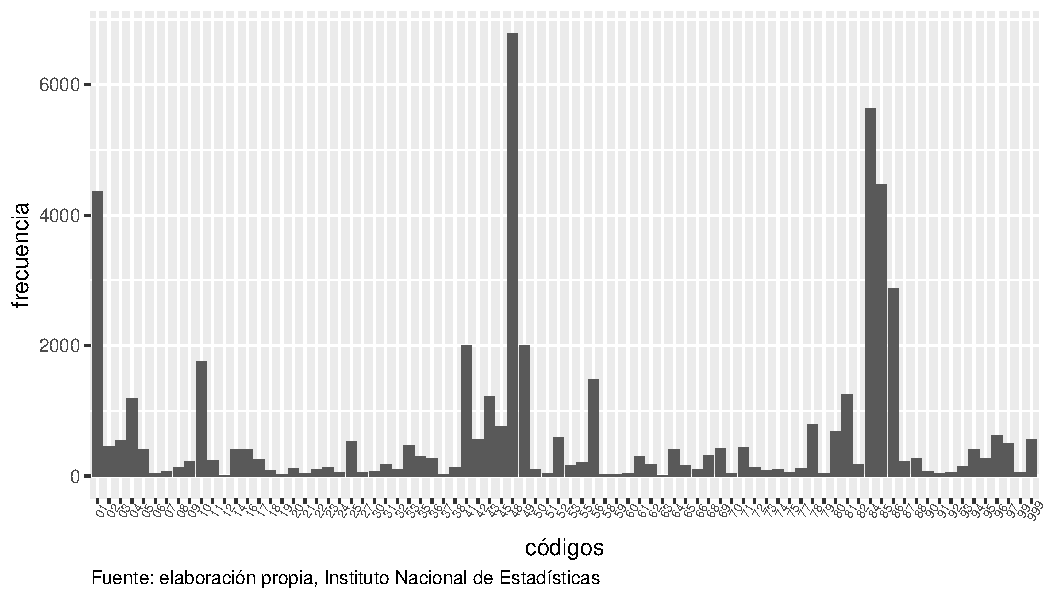
\includegraphics[width = \linewidth]{imagenes/distribucion_caenes.pdf}
\normalsize
\end{figure}

La siguiente tabla muestra algunos ejemplos de glosas asociadas al
código 999. Se puede observar que en algunos casos se podría asignar un
código a un dígito, sin embargo, el nivel de detalle exigido por el
clasificador no permite codificar a dos dígitos.

\begin{table}[H]

\caption{\label{tab:glosas 999}\label{cod_999_caenes}Códigos 999 (algunos ejemplos)}
\centering
\fontsize{9.5}{11.5}\selectfont
\begin{tabular}[t]{l}
\toprule
glosa\_caenes\\
\midrule
contratista en la construccion\\
ong. organización no gubernamental\\
telecomunicaciones\\
servicio de alimentos\\
servicios integrales para la mineria\\
\addlinespace
prestadora de servicios a mineras\\
servicios generales\\
contruccion\\
\bottomrule
\multicolumn{1}{l}{\rule{0pt}{1em}Fuente: elaboración propia, Instituto Nacional de Estadísticas }\\
\end{tabular}
\end{table}

Finalmente, se muestra la cantidad y porcentaje de registros
provenientes de recolección de CAPI y PAPI. Tal como se señala en uno de
los apartados iniciales, una preocupación a lo largo de este trabajo ha
sido elaborar conjuntos de entrenamiento que consideren datos generados
a partir de dispositivos móviles. En ese sentido, cerca de un 100\%
corresponde a levantamientos via tablet, pero dado que algunas
categorías presentaban una escasa presencia, se tomó la decisión de
incorporar algunas glosas del levantamiento de 2018, de modo de abultar
dichas categorías y mejorar el proceso de entrenamiento.

\begin{table}[H]

\caption{\label{tab:unnamed-chunk-1}\label{capi_papi}Procedencia CAPI y PAPI}
\centering
\fontsize{9.5}{11.5}\selectfont
\begin{tabular}[t]{ccc}
\toprule
levantamiento & frecuencia & porcentaje\\
\midrule
capi & 50.749 & 99.1\\
papi & 464 & 0.9\\
\bottomrule
\multicolumn{3}{l}{\rule{0pt}{1em}Fuente: elaboración propia, Instituto Nacional de Estadísticas }\\
\end{tabular}
\end{table}

\hypertarget{dataset-ciuo-08.cl-1}{%
\subsection{Dataset CIUO-08.CL}\label{dataset-ciuo-08.cl-1}}

Para el caso de CIUO-08.CL, el set de datos está conformado por 33.846
registros. El motivo de que la cantidad de registros sea menor a la de
CAENES es la mayor complejidad que tiene este clasificador, lo que tiene
un efecto en la cantidad de glosas diarias que una persona puede
etiquetar. Cabe señalar que al igual que en el caso de CAENES, existen
glosas que presentan valor ``88''. La siguiente tabla muestra la
cantidad de registros con valores 88 en las variables oficio y tarea.
Además, se indica el número de registros en los que tanto oficio como
tarea tienen valor 88. Se observa que el total de registros válidos es
33.823.

\begin{table}[H]

\caption{\label{tab:ciuo valores missing}\label{missing_ciuo}Cantidad valores perdidos CIUO-08.CL}
\centering
\fontsize{9.5}{11.5}\selectfont
\begin{tabular}[t]{lll}
\toprule
missing & frecuencia & porcentaje\\
\midrule
missing oficio & 1 & 0,0\\
missing oficio y tareas & 4 & 0,0\\
missing tareas & 18 & 0,1\\
válido & 33.823 & 99,9\\
\bottomrule
\multicolumn{3}{l}{\rule{0pt}{1em}Fuente: elaboración propia, Instituto Nacional de Estadísticas }\\
\end{tabular}
\end{table}

Respecto al origen de la codificación, la siguiente tabla da cuenta de
que el 63,8\% de los registros fueron codificados en el marco del
Proyecto Estratégico Servicios Compartidos.

\begin{table}[H]

\caption{\label{tab:crear tabla origen ciuo}\label{origen_ciuo}Origen de la codificación CIUO-08.CL}
\centering
\begin{tabu} to \linewidth {>{\raggedright}X>{\raggedright}X>{\raggedright}X}
\toprule
origen & frecuencia & porcentaje\\
\midrule
ene & 12.250 & 36,2\\
sscc & 21.573 & 63,8\\
\bottomrule
\multicolumn{3}{l}{\rule{0pt}{1em}Fuente: elaboración propia, Instituto Nacional de Estadísticas }\\
\end{tabu}
\end{table}

El siguiente gráfico muestra la distribución de la variable CIUO a dos
dígitos. Al igual que en el caso de CAENES, los valores 999 corresponden
a glosas cuya información no permitía llevar a cabo una codificación
adecuada a dos dígitos. La categoría 999 corresponde al 0,4\% del total.

\begin{figure}[H]
\centering
\large
\caption{Distribución de códigos CIUO-08.CL (2 dígitos)}
\label{ciuo_distancia}
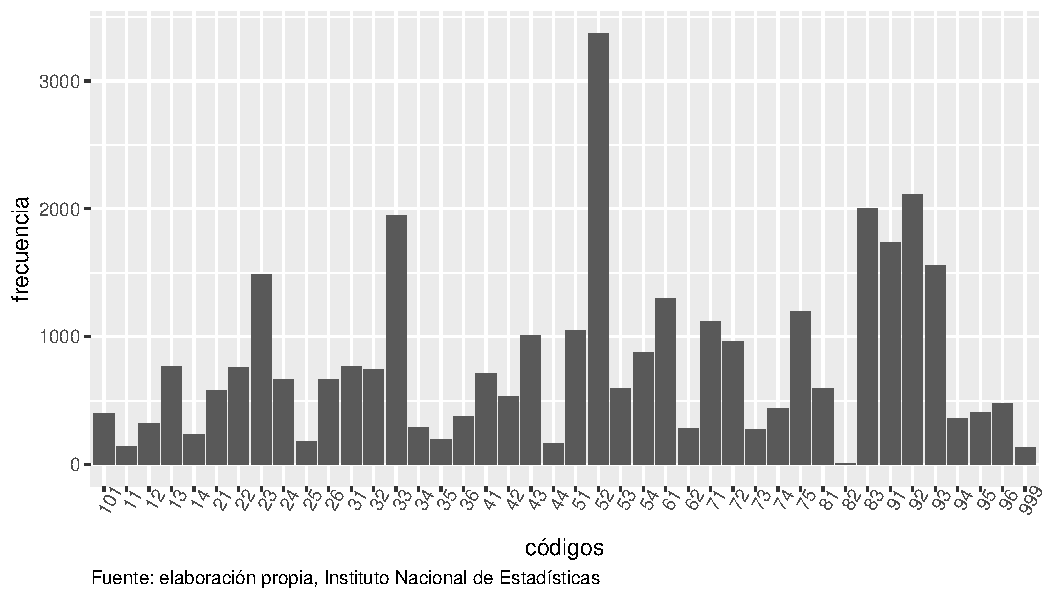
\includegraphics[width = \linewidth]{imagenes/distribucion_ciuo.pdf}
\normalsize
\end{figure}

La siguiente tabla muestra algunos ejemplos de glosas que no pudieron
ser codificadas a dos dígitos debido a la falta de información.

\begin{table}[H]

\caption{\label{tab:glosas 999 ciuo}\label{missing_ciuo_ejemplos}Códigos 999 CIUO (algunos ejemplos)}
\centering
\fontsize{9.5}{11.5}\selectfont
\begin{tabular}[t]{ll}
\toprule
b1\_1 & b1\_2\\
\midrule
informatico & se encarga de\\
auxiliar de escenario & preparar y coordinar los escenarios para actividades, seminarios, reuniones\\
venta de alimentos & preparar, vender alimentos y atención público\\
tecnica en sanitizacion & tramites de empresa\\
empresario & compra y venta de todo tipo de mercadería desde camiones.\\
\addlinespace
supervisor en telecomunicaciones & a cargo de  area telefonia\\
supervisora & supervisar en terreno el desempeño de trabajadores y funcionamiento de maquinarias\\
enfermera naval & realuza atención , control y derivación de pacientes en servicio de urgencias\\
\bottomrule
\multicolumn{2}{l}{\rule{0pt}{1em}Fuente: elaboración propia, Instituto Nacional de Estadísticas }\\
\end{tabular}
\end{table}

\hypertarget{descripciuxf3n-de-los-modelos-de-clasificaciuxf3n}{%
\section{Descripción de los modelos de
clasificación}\label{descripciuxf3n-de-los-modelos-de-clasificaciuxf3n}}

Durante el proceso de entrenamiento se llevó a cabo una serie de
pruebas, con el objeto de encontrar el mejor modelo posible. A grandes
rasgos, se utilizaron variantes para 2 partes del entrenamiento: 1)
metodología para convertir textos en vectores y 2) arquitectura del
algoritmo para hacer el entrenamiento. Si bien existen otras partes del
entrenamiento que pueden impactar en el resultado final, las 2
seleccionadas son las que probablemente tengan un mayor efecto. A raíz
de ello, se priorizó por ellas.

\hypertarget{metodologuxeda-para-vectorizar-textos}{%
\subsection{Metodología para vectorizar
textos}\label{metodologuxeda-para-vectorizar-textos}}

Para que los datos de texto sean procesados por cualquier algoritmo, se
requiere que estos sean convertidos a algún tipo de representación
numérica. Para llevar a cabo esta trasformación existen diferentes
estrategias. Dos de las más importantes son \emph{bag of words (BOW)} y
\emph{word embeddings}. En el caso de BOW es posible encontrar una serie
de variantes, desde el enfoque más simple consistente en identificar la
presencia o ausencia de una palabra, hasta representaciones más
complejas, como tf-idf, que buscan ponderar las palabras de acuerdo a la
importancia que estas tienen en un determinado corpus. La segunda
vertiente, \emph{word embeddings}, consiste en utilizar representaciones
vectoriales de cada palabra, provenientes de un entrenamiento realizado
con grandes volúmenes de texto. Típicamente, se utilizan vectores de 300
dimensiones entrenados con toda la información existente en wikipedia
o/y otras fuentes similares\footnote{Existe abundante literatura
  respecto a \emph{word embeddings}. Para una introducción al tema,
  revisar los libros \emph{Introduction to Deep Learning} (Aggarwal, C
  2018) y \emph{Neural Networks and Deep Learning} (Skansi, S 2018).}.

Dado que cada palabra de un texto es representada por un vector, se hace
necesario alguna medida sintética que permita llegar a una
representación para el texto completo. Para ello, existen distintas
estrategias y lo que se utilizó en este trabajo fue la media de cada una
de las 300 dimensiones. Así, cada glosa es representada por un vector de
300 dimensiones. Dicho vector contiene la información ``resumida'' de
las palabras que componen cada glosa.

En el marco de este trabajo se llevaron a cabo pruebas con ambos
enfoques.

\begin{itemize}
\tightlist
\item
  Estrategia BOW: Dentro de la estrategia BOW se utilizaron 2 variantes.
  En primer lugar, se construyeron vectores utilizando tf-idf. Ello
  permite extraer de mejor manera el ``significado'' de cada palabra,
  que utilizando únicamente la presencia o ausencia. De este modo, un
  texto queda representado por un vector que tiene tantas dimensiones
  como palabras diferentes existan en el corpus. Dado que un texto por
  lo general contiene solo una pequeña fracción del total de palabras
  del vocabulario, el resultado corresponde a una matriz en la que la
  mayoría de sus elementos es 0. Típicamente, seguir esta metodología
  implica construir vectores con varios miles de dimensiones, lo cual
  supone un alto costo de procesamiento, pero dado que la mayor parte de
  los elementos corresponde a valores 0, es posible utilizar algunas
  estrategias para disminuir de manera importante el tiempo de
  ejecución.
\end{itemize}

La segunda variante de BOW utilizada en este trabajo consiste en asociar
cada palabra diferente del corpus a un índice y luego representar cada
texto como una secuencia de índices. Esto quiere decir que un texto con
5 palabras quedará representado por un vector de 5 dimensiones. Es
importante mencionar que dado que los textos no tienen la misma cantidad
de palabras, se debe recurrir a alguna estrategia para que todos los
vectores terminen con la misma cantidad de elementos. Para ello, se
utiliza un procedimiento denominado \emph{padding}, que consiste en
fijar un valor para el largo de los vectores y completar con ceros todos
los vectores que tengan un número menor a dicho valor máximo.

Cabe señalar que en ambos enfoques de BOW la ``semántica'' de las
palabras proviene de la información presente en el set de datos que se
utiliza para el entrenamiento. En ese sentido, no se recurre a
información externa, lo cual si ocurre en el enfoque basado en
\emph{word embeddings}.

\begin{itemize}
\tightlist
\item
  Estrategia \emph{word embedding}: como ya se ha mencionado, \emph{word
  embeddings} es una manera de construir representaciones de palabras
  por medio de un proceso de aprendizaje en el cual se utilizan grandes
  volúmenes de texto. Así, una red neuronal es entrenada para que, a
  partir de una palabra, sea predicho el contexto de la misma o,
  inversamente, el entrenamiento puede realizarse para que a partir de
  un contexto, se prediga una palabra. Cuando este proceso se hace con
  una cantidad de datos suficientes, es posible que la red ``aprenda''
  representaciones de las palabras que capturan su semántica.
\end{itemize}

En el marco de este trabajo se utilizó un modelo entrenado por
\href{https://github.com/dccuchile/spanish-word-embeddings/blob/master/emb-from-suc.md}{Jorge
Perez}. El modelo contiene vectores de 300 dimensiones y su
entrenamiento se hizo mediante el algoritmo FastText.

\hypertarget{arquitecturas-probadas}{%
\subsection{Arquitecturas probadas}\label{arquitecturas-probadas}}

Durante la etapa de pruebas, se llevaron a cabo ejercicios con 2
arquitecturas de redes neuronales. Dichas arquitecturas se probaron con
las dos estrategias de vectorización mencioandas más arriba, a partir de
lo cual se originan 4 modelos diferentes.

Las arquitecturas consideradas fueron \emph{feed-forward} y \emph{gated
recurrent unit} (GRU). La arquitectura de red \emph{feed-forward} es la
configuración más sencilla de redes neuronales y se incorpora en este
trabajo con el objeto de contar con una medida base contra la cual
contrastar otras arquitecturas de redes más complejas. Por su parte, las
redes GRU son una variante de la arquitectura LSTM (\emph{Long
short-term memory}), pero con una estructura más simple y, por ende, con
una menor cantidad de parámetros a estimar.

Ambas arquitecturas (LSTM y GRU) comparten la característica de permitir
que parte de la información inicial de una secuencia de datos es
traspasada hacia los estados posteriores, combatiendo el problema de la
``falta de memoria'' de largo plazo. En ese sentido, la arquitectura GRU
es sumamente útil para procesar datos de texto, ya que el lenguaje
humano puede ser entendido como una secuencia de elementos concatenados,
en los que cierto orden genera sentido.

\hypertarget{resultados-del-entrenamiento}{%
\subsubsection{Resultados del
entrenamiento}\label{resultados-del-entrenamiento}}

Los cuadros siguientes resumen los resultados obtenidos en el set de
testeo para cada una de las estrategias y desagregaciones realizadas. Es
importante mencionar que los modelos fueron entrenados con un
subconjunto de los datos, ya que solo se utilizaron aquellos
\textbf{etiquetados por codificadores de SSCC}, dejando fuera aquellos
provenientes del control de calidad de la ENE\footnote{La variable
  origen permite filtrar los datos etiquetados por el equipo de SSCC.}.
Respecto a la partición de los datos, se llevó a cabo un entrenamiento
con el 80\% de cada uno de los datasets elaborados. Dentro de dicho 80\%
se seleccionó un 10\% para hacer la validación durante el entrenamiento.

En el caso de CAENES no se advierten diferencias importantes entre las
distintas estrategias elegidas, sin embargo, vale la pena mencionar que
tanto a uno como a dos dígitos, la vectorización mediante secuencias
(seq\_1d y seq\_2d) muestra un desempeño ligeramente más alto que los
demás modelos. Esto se debe a que en la extracción de características
para esa estrategia, se utilizó la información de la variable CISE, lo
cual no tiene demasiado sentido en un modelo que incorpore \emph{word
embeddings}, puesto que habría supuesto encontrar representaciones
vectoriales para las categorías de CISE, cuyo significado está definido
específicamente para la variable en cuestión\footnote{La variable CISE
  está conformada por categorías numéricas que tienen sentido en el
  contexto específico de dicha variable. Por ejemplo, el caracter ``1''
  tiene unsignificado muy particular, pues está asociado a los
  empleadores. Ahora bien, dado que el modelo de \emph{embeddings}
  contiene el ``significado general'' de ``1'', el vector asignado a ese
  caracter no apuntará en una dirección similar a la que ``1'' tiene
  para la variable CISE.}. Pese a ello, se recomienda que el modelo
basado en \emph{word embeddings} sea utilizado de manera productiva, ya
que el hecho de enriquecer la descripción de los textos mediante un
modelo entrenado con grandes cantidades de texto, hace suponer que las
predicciones sean menos sensibles a cambios en la manera de registrar la
información.\footnote{Para mayores detalles sobre la construcción de
  \emph{word embeddings}, ver el trabajo de Jorge Perez Rojas
  {[}\url{https://github.com/dccuchile/spanish-word-embeddings}{]}}
Adicionalmente, es relevante mencionar que un modelo que utilice
únicamente la información contenida en la glosa es más deseable que uno
que contenga variable auxiliares, ya que ello hace posible que sea
utilizado en un mayor número de situaciones. La razón es que las
preguntas de ocupación y actividad económica tienen un nivel elevado de
estandarización a través de las distintas encuestas de hogares dentro
del INE. Al contrario, las variables auxiliares que acompañan a las
glosas dependen de los objetivos particulares de cada estudio y no
siempre están presentes en todos los cuestionarios.

En el caso de CIUO es un poco más evidente que el modelo que utiliza
\emph{word embeddings} presenta un mejor rendimiento que los demás, por
lo que, nuevamente, se sugiere que sea utilizado de manera productiva.

\begin{table}[H]

\caption{\label{tab:unnamed-chunk-2}Resultados CAENES 1 dígito}
\centering
\fontsize{9.5}{11.5}\selectfont
\begin{tabular}[t]{lrrrr}
\toprule
modelo & acc & macro & micro & weighted\\
\midrule
seq\_1d & 0.9384 & 0.8757 & 0.9384 & 0.9386\\
tfidf\_1d & 0.9327 & 0.8658 & 0.9327 & 0.9330\\
emb\_simple\_1d & 0.9274 & 0.8641 & 0.9274 & 0.9280\\
emb\_gru\_1d & 0.9327 & 0.8694 & 0.9327 & 0.9328\\
\bottomrule
\multicolumn{5}{l}{\rule{0pt}{1em}Fuente: elaboración propia, Instituto Nacional de Estadísticas }\\
\end{tabular}
\end{table}

\begin{table}[H]

\caption{\label{tab:unnamed-chunk-2}Resultados CAENES 2 dígito}
\centering
\fontsize{9.5}{11.5}\selectfont
\begin{tabular}[t]{lrrrr}
\toprule
modelo & acc & macro & micro & weighted\\
\midrule
seq\_2d & 0.9075 & 0.7536 & 0.9075 & 0.9083\\
tfidf\_2d & 0.9076 & 0.7579 & 0.9076 & 0.9081\\
emb\_simple\_2d & 0.9021 & 0.7631 & 0.9021 & 0.9039\\
emb\_gru\_2d & 0.9048 & 0.7630 & 0.9048 & 0.9052\\
\bottomrule
\multicolumn{5}{l}{\rule{0pt}{1em}Fuente: elaboración propia, Instituto Nacional de Estadísticas }\\
\end{tabular}
\end{table}

\begin{table}[H]

\caption{\label{tab:unnamed-chunk-2}Resultados CIUO 1 dígito}
\centering
\fontsize{9.5}{11.5}\selectfont
\begin{tabular}[t]{lrrrr}
\toprule
modelo & acc & macro & micro & weighted\\
\midrule
seq\_1d & 0.8858 & 0.8599 & 0.8858 & 0.8855\\
tfidf\_1d & 0.8684 & 0.8362 & 0.8684 & 0.8686\\
emb\_simple\_1d & 0.8793 & 0.8519 & 0.8793 & 0.8807\\
emb\_gru\_1d & 0.8989 & 0.8796 & 0.8989 & 0.8990\\
\bottomrule
\multicolumn{5}{l}{\rule{0pt}{1em}Fuente: elaboración propia, Instituto Nacional de Estadísticas }\\
\end{tabular}
\end{table}

\begin{table}[H]

\caption{\label{tab:unnamed-chunk-2}Resultados CIUO 2 dígito}
\centering
\fontsize{9.5}{11.5}\selectfont
\begin{tabular}[t]{lrrrr}
\toprule
modelo & acc & macro & micro & weighted\\
\midrule
seq\_2d & 0.8456 & 0.7249 & 0.8456 & 0.8476\\
tfidf\_2d & 0.8412 & 0.7355 & 0.8412 & 0.8431\\
emb\_simple\_2d & 0.8324 & 0.7220 & 0.8324 & 0.8348\\
emb\_gru\_2d & 0.8526 & 0.7364 & 0.8526 & 0.8543\\
\bottomrule
\multicolumn{5}{l}{\rule{0pt}{1em}Fuente: elaboración propia, Instituto Nacional de Estadísticas }\\
\end{tabular}
\end{table}

\newpage

\hypertarget{modelos-en-producciuxf3n}{%
\section{Modelos en producción}\label{modelos-en-producciuxf3n}}

El presente proyecto pone a disposición de los usuarios el código fuente
(scripts en R y Python) y los datos necesarios para reproducir los
resultados presentados más arriba, de manera tal de transparentar las
decisiones metodológicas y abrir el espacio para futuras mejoras. Ahora
bien, para reproducir completamente los resultados es necesario que los
y las usuarias cuenten con una serie de componentes, lo cual no siempre
es una tarea sencilla. De manera esquemática, se presentan las
principales herramientas necesarias para ejecutar las rutinas:

\begin{itemize}
\tightlist
\item
  R y RStudio
\item
  Python
\item
  Reticulate
\item
  Keras/Tensorflow
\end{itemize}

Además de lo anterior, es necesario considerar que el entrenamiento de
los modelos fue realizado en un sistema operativo Linux y hasta el
momento se ha probado que las rutinas se ejecuten correctamente en las
distribuciones CENTOS y Ubuntu y no se han realizado pruebas en Windows.
Adicionalmente, se utilizó un \emph{virtual env} de Python, para
facilitar la vinculación entre R y Python. Las dependencias señaladas
más arriba, sumado a ciertas decisiones (sistema operativo Linux y
vinculación de R con Python) suponen una barrera de entrada importante
para que los modelos sean utilizados con fluidez.

Con el objeto de que la codificación automática sea utilizada por la
mayor cantidad de usuarios y usuarias posible, se pone a diposición una
API (\emph{Application Programming Interface}), que posibilita que los
modelos de clasificación sean utilizados de manera relativamente
sencilla. Una API permite que un usuario o usuaria se comunique con un
servicio, sin la necesidad de conocer los detalles de la implementación
que hay detrás de dicho servicio. Basta con que una solicitud
(\emph{request}) sea realizada con cierta estructura, para que la API
retorne un resultado, que también cumple con cierta estructura. En ese
sentido, la API que se pone a disposición permite que los modelos sean
utilizados, sin que las y los usuarios cuente con ninguno de los
requerimientos mencionados más arriba, disminuyendo de manera
significativa las barreras de entrada.

En ese sentido, desde el punto de vista de un analista, la única
herramienta que se requiere para poder utilizar los modelos es alguna
librería que permita hacer solicitudes a un servidor. Independientemente
de la herramienta utilizada para hacer la solicitud, la API retornará la
predicción del modelo en formato json, el cual es fácilmente manipulable
en casi cualquier lenguaje de programación.

A continuación se presenta un ejemplo de cómo interactuar con la API
mediante el paquete \texttt{httr} de \texttt{R}. El primer parámetro del
\emph{request} corresponde al servidor y al \emph{endpoint} para la
predicción. Dado que no es deseable migrar la API de un servidor a otro,
este parámetro debería permanecer relativamente estable. En segundo
lugar, debe indicarse que se trata de un archivo json, lo cual también
debiese ser algo que no sufra variaciones. Dentro del cuerpo del
\emph{request} debe indicarse cuáles son los textos para los cuales se
requiere una predicción. En este caso se están enviando al servidor las
10 primeras glosas de la columnaa \emph{glosa\_caenes}, lo que quiere
decir que previo a la solicitud, deben estar cargadas en el ambiente las
glosas a utilizar. Adicionalmente, debe indicarse si los datos
corresponden a ocupación o actividad económica, mediante los strings
\emph{caenes} o \emph{ciuo}. Finalmente, se debe indicar si la
predicción se requiere a uno o dos dígitos.

Se puede observar que para cada glosa el servidor retorna 3 elementos:
codigo\_int, cod\_final y prob.El primero de estos elementos no tiene
demasiada utilidad para el usuario, ya que refiere a un identificador
interno de la API. El segundo corresponde al código predicho por el
modelo. El tercer elemento es la probabilidad que la red asignó al
código predicho y puede ser utilizado como un \emph{proxy} de certeza.
Así, valores cercanos a uno corresponden a una alta seguridad asignada
por la red al momento de seleccionar el código. A la inversa, valores
cercanos a 0 pueden ser interpretados como una predicción de baja
certeza.

\begin{Shaded}
\begin{Highlighting}[]
\CommentTok{# Predecir a un dígito}
\KeywordTok{library}\NormalTok{(httr)}
\KeywordTok{library}\NormalTok{(feather)}
\NormalTok{caenes <-}\StringTok{ }\KeywordTok{read_feather}\NormalTok{(}\StringTok{"src/data/split_train_test/test.feather"}\NormalTok{)}
\NormalTok{request <-}\StringTok{  }\NormalTok{httr}\OperatorTok{::}\KeywordTok{POST}\NormalTok{(}\StringTok{"http://143.198.79.143:8080/predict"}\NormalTok{,}
                 \DataTypeTok{encode =} \StringTok{"json"}\NormalTok{,}
                 \DataTypeTok{body =}  \KeywordTok{list}\NormalTok{(}\DataTypeTok{text =}\NormalTok{ caenes}\OperatorTok{$}\NormalTok{glosa_caenes[}\DecValTok{1}\OperatorTok{:}\DecValTok{10}\NormalTok{],}
                              \DataTypeTok{classification =} \StringTok{"caenes"}\NormalTok{,}
                              \DataTypeTok{digits =} \DecValTok{1}\NormalTok{)}
\NormalTok{)}

\CommentTok{# Revisar el status}
\NormalTok{httr}\OperatorTok{::}\KeywordTok{status_code}\NormalTok{(request)}
\end{Highlighting}
\end{Shaded}

\begin{verbatim}
## [1] 200
\end{verbatim}

\begin{Shaded}
\begin{Highlighting}[]
\CommentTok{# Extraer el contenido }
\NormalTok{response <-}\StringTok{ }\NormalTok{httr}\OperatorTok{::}\KeywordTok{content}\NormalTok{(request)}

\CommentTok{# Impimir las dos primeras predicciones}
\NormalTok{tabla <-}\StringTok{ }\KeywordTok{map}\NormalTok{(response[}\DecValTok{1}\OperatorTok{:}\DecValTok{5}\NormalTok{], as.data.frame) }\OperatorTok\StringTok{ }
\StringTok{  }\KeywordTok{bind_rows}\NormalTok{()}
\end{Highlighting}
\end{Shaded}

\begin{table}[H]

\caption{\label{tab:tabla_api}Resultado de una consulta}
\centering
\fontsize{9.5}{11.5}\selectfont
\begin{tabular}[t]{ccc}
\toprule
codigo\_int & cod\_final & prob\\
\midrule
0 & A & 0.9989\\
14 & O & 0.9745\\
5 & F & 0.9997\\
13 & N & 0.9999\\
2 & C & 0.9973\\
\bottomrule
\multicolumn{3}{l}{\rule{0pt}{1em}Fuente: elaboración propia, Instituto Nacional de Estadísticas }\\
\end{tabular}
\end{table}

\newpage

\hypertarget{conclusiones-y-recomendaciones}{%
\section{Conclusiones y
recomendaciones}\label{conclusiones-y-recomendaciones}}

El presente proyecto ha tenido el objetivo de generar datos de
entrenamiento y modelos para ser utilizados libremente por la
institución. En ese sentido, este esfuerzo se enmarca en un camino que
la institución viene recorriendo desde hace algunos años hacia la
automatización de procesos de codificación. En este camino, el enfoque
de \emph{machine learning} ha generado resultados positivos y es de
esperar que su utilización siga expandiéndose con el paso del tiempo.
Ahora bien, al mismo tiempo en que se llevan a cabo avances en el campo
de la inteligencia artificial, surgen nuevos desafíos institucionales,
que no deben ser soslayados.

\begin{itemize}

  \item En primer lugar, es sumamente importante considerar que la continuidad operativa de los modelos puestos a disposición requiere de un equipo que pueda hacerse cargo del monitoreo y actualizaciones que el sistema requiera. En ese sentido, la Sección de Nomenclaturas surge como la unidad más idónea para llevar a cabo dicha tarea, ya que en ella recae la responsabilidad de implementar los estándares internacionales de los clasificadores a la realidad nacional. Este equipo debiese encargarse de actualizar constantemente los sets de entrenamiento, a partir de las auditorias y/o revisiones realizadas a los productos de la institución. Lo anterior implica poner en marcha un flujo constante, lo cual haría posible una mejora continua de la calidad de los datos. Es importante mencionar que la actualización constante de los sets de entrenamiento no supone un aumento de costos relevante para la institución, ya que al ser las auditorías parte del quehacer cotidiano del INE, se hace necesario únicamente adecuar algunos flujos de trabajo para sacar provecho de un trabajo que los equipos ya están llevando a cabo.  

  \item A lo largo de este documento se ha mencionado la necesidad de monitoreo constante de los modelos. Tal como se ha señalado antes, una estrategia basada en una revisión manual por parte de analistas especializados es efectiva, sin embargo, conlleva costos elevados. En ese sentido, una estrategia automática de seguimiento constituiría una herramienta útil para mejorar y facilitar la continuidad operativa de los modelos en producción. Esto podría ser pensado como un mecanismo automático, que genere alertas cuando exista probabilidad de que un modelo comience a fallar. 

  \item De lo anterior se desprende la necesidad de llevar a cabo nuevos entrenamientos cada vez que sea necesario o cada vez que el aumento de datos haga pensar que es posible mejorar el rendimiento actual de los modelos. Se propone que la responsabilidad de llevar a cabo este trabajo, al igual que el de mantenimiento de los datasets de entrenamiento, recaiga en la Sección de Nomenclaturas. Este equipo es el más indicado para evaluar si un modelo está funcionando adecuadamente e identificar cuáles son las falencias que aquel pueda tener.       

  \item Se ha mencionado que modificaciones abruptas en las metodologías de levantamiento pueden generar una caída relevante en el rendimiento de un algoritmo, ya que podrían alterar la manera en la que los datos son registrados, produciéndose una distancia respecto a los datos que se utilizaron durante el entrenamiento. Ello quiere decir que cada vez que un modelo de clasificación esté en producción, debiese estar presente la preocupación sobre cuáles podrían ser los cambios en la manera en la que los datos son registrados. En ese sentido, una estandarización de las preguntas sobre ocupación y actividad económica aparece como algo de gran importancia. Es posible que debido a las particularidades de algún producto, sea necesario modificar o diminuir la cantidad de preguntas para registar ocupación y/o actividad económica. El costo de ello, además de perder comparabilidad con otros estudios, es limitar severamente la posibilidad de utilizar modelos ya entrenados para una tarea. En ese sentido, de ser posible es altamente recomendable que tanto las baterías como los fraseos de las preguntas se asemejen los más posible al modo en el que actualmente los cuestionarios del INE consultan ocupación y actividad económica.       

  \item Es importante mencionar que cualquier estrategia basada en *machine learning* debiese considerar una parte de trabajo manual. Los objetivos institucionales imponen la necesidad de velar por un uso eficiente de los recursos, sin embargo, ello no debería comprometer la calidad. Dado que cualquier método de codificación basado en *machine learning* introduce un porcentaje de error, el objetivo debiese ser minimizarlo al menor costo posible. En ese sentido, el etiquetado manual de una fracción de los datos, supone un complemento muy importante en una estrategia mayormente automatizada. Siempre existirán glosas complejas o que simplemente no han estado presentes durante el entrenamiento. Para esos casos particulares, el trabajo manual suele tener resultados mucho mejores que un algoritmo. El desafío consiste, entonces, en discriminar cuáles son las glosas que requieren ser codificadas manualmente. Un camino posible es utilizar la probabilidad de respuesta que entregan los modelos (ver capítulo sobre la puesta en producción) y considerar que dicha variable es un *proxy* de dificultad. Si efectivamente dicha probabilidad da cuenta de la dificultad de codificación de las glosas, es posible ordenarlas de menor a mayor complejidad y establecer un punto de corte que permita separar los registros que serán codificados por un modelo de aquellos que serán revisados por una persona experta.
\newline
\newline Con el objeto de ejemplificar cómo funciona la estrategia, el siguiente gráfico muestra la relación entre el error de predicción y el porcentaje de registros codificados automáticamente, para lo cual se utilizaron datos de la Encuesta de Presupuestos Familiares. Se puede observar que, como es de esperar, conforme aumenta el porcentaje de codificación manual, disminuye el error de predicción y, lo que es más importante, dicha reducción avanza a tasas decrecientes. Expresado de otro modo, los primeros registros que se codifican manualmente generan un "retorno" importante, el cual va disminuyendo progresivamente conforme avanza el porcentaje de datos codificados manualmente. Esto es un indicio de que el ordenamiento generado a partir del *proxy* de dificutad funciona, ya que si aquel fuese totalmente aleatorio, se observaría una reducción del error, pero dicha reducción no tendría la forma observada en el gráfico.
\newline
\newline Una vez construida la relación entre error y codificación manual, es posible escoger un punto de corte, con el objeto de aproximar cuál será el porcentaje de error que introducirá la codificación automática. A partir de la relación descrita se desprende una decisión de costo/beneficio, ya que el error puede ser entendido como una función de los recursos destinados a codificar registros manualmente. Así, codificar automáticamente los primeros registros genera un beneficio importante, pero avanzar hacia un error 0 se torna cada vez más costoso. A raíz de ello podría llegarse a la determinación de tolerar cierto porcentaje de error. En el caso de este ejemplo se seleccionó un porcentaje de codificación de 5%, valor que no debe ser interpretado como una recomendación, sino simplemente como un número arbitrario para mostrar el funcionamiento de la estrategia.         


\begin{figure}[H]
\centering
\large
\caption{Relación entre codificación manual y automática (Datos EPF)}
\label{manual_vs_automatico}
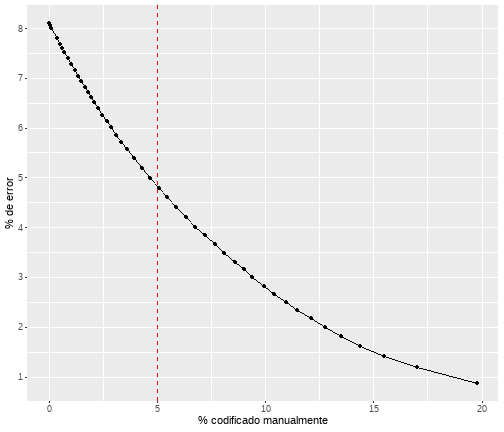
\includegraphics[width=0.7\columnwidth]{imagenes/manual_vs_automatico.png}
\normalsize
\end{figure}


  \item Finalmente, debe subrayarse que la pertinencia de los métodos de codificación basados en *machine learning* siempre debe ser evaluada a la luz de las necesidades y restricciones de cada operación. Así, para productos que son estables en el tiempo, como las operaciones coyunturales, una estrategia de este tipo resulta de gran utilidad, ya que al no existir modificaciones importantes en la metodología, un mismo entrenamiento puede ser usado muchas veces, lo cual implica un ahorro importante de recursos. Por otro lado, encuestas estructurales pueden no verse tan beneficiadas de un método como este, puesto que debido a la periodicidad con la que se realizan, es altamente probable que entre una versión y otra se produzcan cambios metodológicos importantes, que dejen obsoletos los sets de entrenamiento. Bajo una estrategia de *machine learning*,  dichos cambios obligarían a actualizar los sets de entrenamiento mediante la recodificación manual de un gran número de casos, poniendo en duda su utilidad como método de ahorro de costos. Este tipo de obsolescencia, sin embargo, impacta de forma más directa a las operaciones estadísticas que implementan clasificadores que no se ven afectos a actualización continua, como es el caso del Clasificador de Consumo Individual por Finalidades (CCIF). En el caso de los clasificadores CIUO-08.CL y CAENES, esta actualización es constante.

 \item Para los Censos de Población y Vivienda se recomienda altamente el uso de metodologías de *machine Learning* para la codificación de ocupación y actividad económica, considerando el tamaño de la operación estadística, el ahorro de costos y la mejora en oportunidad que podría retornar este tipo de estrategia.

\end{itemize}

\newpage

\hypertarget{referencias}{%
\section*{Referencias}\label{referencias}}
\addcontentsline{toc}{section}{Referencias}

\hypertarget{refs}{}
\leavevmode\hypertarget{ref-aggarwal}{}%
Aggarwal, C. 2018. \emph{Neural Networks and Deep Learning}. Springer.

\leavevmode\hypertarget{ref-guerrero_cabezas}{}%
Cabezas, J. y Guerrero, J. 2019. «Clasificación automática de textos
utilizando técnicas de text mining: Aplicación a las glosas de la
Encuesta Nacional de Empleo (ENE)». Documento de Trabajo.
\url{https://www.ine.cl/docs/default-source/documentos-de-trabajo/clasificacion-automatica-de-textos-utilizando-tecnicas-de-text-mining-aplicacion-a-las-glosas-de-la-encuesta-nacional-de-empleo.pdf?sfvrsn=1ddfe7d2_2}.

\leavevmode\hypertarget{ref-ine_caenes}{}%
INE. 2016. «Clasificador de Actividades Económicas Nacional para
Encuestas Sociodemográficas». Documento de Trabajo.
\url{https://www.ine.cl/docs/default-source/ocupacion-y-desocupacion/metodologia/espanol/documento-clasificador-de-rama-de-actividad-econ\%C3\%B3mica-caenes-(abril-2016).pdf?sfvrsn=1b1cc016_3?len=en}.

\leavevmode\hypertarget{ref-codificacion_ene}{}%
---------. 2019. «Sistema de clasificación y codificación automatica en
la encuesta nacional de empleo». Documento de Trabajo.
\url{https://www.ine.cl/docs/default-source/ocupacion-y-desocupacion/metodologia/espanol/documento-sistema-de-clasificaci\%C3\%B3n-y-codificaci\%C3\%B3n-autom\%C3\%A1tica-(mayo-2019).pdf?sfvrsn=ceea6423_3}.

\leavevmode\hypertarget{ref-skansi}{}%
Skansi, S. 2018. \emph{Introduction to Deep Learning. From Logical
Calculus to Artificial Intelligence}. Springer.

\end{document}
